\begin{figure*}[t]
    \centering
    \begin{subfigure}[b]{.12\textwidth}
        \centering
        \includegraphics[width=\linewidth]{figure/plot/reference/fig12-side-sql-u1.pdf}
        \caption{[Ref] U1}
        \label{fig:12:ref:side-channel-feature-u1}
    \end{subfigure}
    \hfill
    \begin{subfigure}[b]{.12\textwidth}
        \centering
        \includegraphics[width=\linewidth]{figure/plot/reference/fig12-side-sql-u2.pdf}
        \caption{[Ref] U2}
        \label{fig:12:ref:side-channel-feature-u2}
    \end{subfigure}
    \hfill
    \begin{subfigure}[b]{.12\textwidth}
        \centering
        \includegraphics[width=\linewidth]{figure/plot/reference/fig12-side-sql-c1.pdf}
        \caption{[Ref] C1}
        \label{fig:12:ref:side-channel-feature-c1}
    \end{subfigure}
    \hfill
    \begin{subfigure}[b]{.12\textwidth}
        \centering
        \includegraphics[width=\linewidth]{figure/plot/reference/fig12-side-sql-c2.pdf}
        \caption{[Ref] C2}
        \label{fig:12:ref:side-channel-feature-c2}
    \end{subfigure}
    \hfill
    \begin{subfigure}[b]{.12\textwidth}
        \centering
        \includegraphics[width=\linewidth]{figure/plot/reference/fig12-side-sql-c3.pdf}
        \caption{[Ref] C3}
        \label{fig:12:ref:side-channel-feature-c3}
    \end{subfigure}
    \hfill
    \begin{subfigure}[b]{.12\textwidth}
        \centering
        \includegraphics[width=\linewidth]{figure/plot/reference/fig12-side-sql-q1.pdf}
        \caption{[Ref] Q1}
        \label{fig:12:ref:side-channel-feature-q1}
    \end{subfigure}
    \hfill
    \begin{subfigure}[b]{.12\textwidth}
        \centering
        \includegraphics[width=\linewidth]{figure/plot/reference/fig12-side-sql-i1.pdf}
        \caption{[Ref] I1}
        \label{fig:12:ref:side-channel-feature-i1}
    \end{subfigure}
    \hfill
    \begin{subfigure}[b]{.12\linewidth}
        \centering
        \includegraphics[width=\linewidth]{figure/plot/reference/fig12-side-sql-s1.pdf}
        \caption{[Ref] S1}
        \label{fig:12:ref:side-channel-feature-s1}
    \end{subfigure}
    \\
    \begin{subfigure}[b]{.12\textwidth}
        \centering
        \resizebox{\linewidth}{!}{\includegraphics{example-image-duck}}
        % \includegraphics[width=\linewidth]{figure/plot/reproduce/fig12-side-sql-u1.pdf}
        \caption{[Rep] U1}
        \label{fig:12:rep:side-channel-feature-u1}
    \end{subfigure}
    \hfill
    \begin{subfigure}[b]{.12\textwidth}
        \centering
        \resizebox{\linewidth}{!}{\includegraphics{example-image-duck}}
        % \includegraphics[width=\linewidth]{figure/plot/reproduce/fig12-side-sql-u2.pdf}
        \caption{[Rep] U2}
        \label{fig:12:rep:side-channel-feature-u2}
    \end{subfigure}
    \hfill
    \begin{subfigure}[b]{.12\textwidth}
        \centering
        \resizebox{\linewidth}{!}{\includegraphics{example-image-duck}}
        % \includegraphics[width=\linewidth]{figure/plot/reproduce/fig12-side-sql-c1.pdf}
        \caption{[Rep] C1}
        \label{fig:12:rep:side-channel-feature-c1}
    \end{subfigure}
    \hfill
    \begin{subfigure}[b]{.12\textwidth}
        \centering
        \resizebox{\linewidth}{!}{\includegraphics{example-image-duck}}
        % \includegraphics[width=\linewidth]{figure/plot/reproduce/fig12-side-sql-c2.pdf}
        \caption{[Rep] C2}
        \label{fig:12:rep:side-channel-feature-c2}
    \end{subfigure}
    \hfill
    \begin{subfigure}[b]{.12\textwidth}
        \centering
        \resizebox{\linewidth}{!}{\includegraphics{example-image-duck}}
        % \includegraphics[width=\linewidth]{figure/plot/reproduce/fig12-side-sql-c3.pdf}
        \caption{[Rep] C3}
        \label{fig:12:rep:side-channel-feature-c3}
    \end{subfigure}
    \hfill
    \begin{subfigure}[b]{.12\textwidth}
        \centering
        \resizebox{\linewidth}{!}{\includegraphics{example-image-duck}}
        % \includegraphics[width=\linewidth]{figure/plot/reproduce/fig12-side-sql-q1.pdf}
        \caption{[Rep] Q1}
        \label{fig:12:rep:side-channel-feature-q1}
    \end{subfigure}
    \hfill
    \begin{subfigure}[b]{.12\textwidth}
        \centering
        \resizebox{\linewidth}{!}{\includegraphics{example-image-duck}}
        % \includegraphics[width=\linewidth]{figure/plot/reproduce/fig12-side-sql-i1.pdf}
        \caption{[Rep] I1}
        \label{fig:12:rep:side-channel-feature-i1}
    \end{subfigure}
    \hfill
    \begin{subfigure}[b]{.12\linewidth}
        \centering
        \resizebox{\linewidth}{!}{\includegraphics{example-image-duck}}
        % \includegraphics[width=\linewidth]{figure/plot/reproduce/fig12-side-sql-s1.pdf}
        \caption{[Rep] S1}
        \label{fig:12:rep:side-channel-feature-s1}
    \end{subfigure}

    \caption{Access patterns of database operations. (a)-(h) each shows the access pattern for a database operation: the bottom figure shows the latencies in a concentrated range of iterations and sets, and the top figure shows the latency distributions.}
    \label{fig:12:side-channel-feature}

\end{figure*}
